\section{Audio and Speech Coding}




\begin{questionbox}{Domanda 39}
Explain masking in the auditory system: define frequency masking and \textbf{temporal masking} (pre/post-masking) with their time-scale orders of magnitude.
\end{questionbox}


Auditory masking means that a strong sound can make weaker sounds inaudible. Perceptual audio codecs exploit this by spending fewer bits where \textbf{quantization} noise is hidden below the \textbf{masking threshold}.

Frequency masking is \textbf{simultaneous masking}: a strong component at frequency $f_0$ raises the hearing threshold around nearby frequencies, mostly within the same critical band.

\textbf{temporal masking} happens around the time of a masker:

\begin{itemize}
  \item pre-masking hides sounds shortly before the masker, typically for a few milliseconds;
  \item post-masking hides sounds after the masker, often up to about $100$-$200$ ms depending on level and content.
\end{itemize}



\begin{questionbox}{Domanda 40}
What is the critical band and how does it relate to the audibility condition of a set of sinusoids close in frequency?
\end{questionbox}


A critical band is a frequency interval processed roughly by the same auditory filter in the cochlea. Its bandwidth increases with center frequency.

When several sinusoids are close in frequency, they interact inside the same critical band. Even if each component is individually weak, their combined power can become audible if it exceeds the local hearing threshold. A simplified condition is:


$$
\sum_i g_i^2 > S_0(f_n)
$$


where $g_i^2$ are the sinusoid powers and $S_0(f_n)$ is the absolute hearing threshold near frequency $f_n$.



\begin{questionbox}{Domanda 41}
(A\&S Comp.) Explain the difference between Source-Based (Parametric) coding and Sink-Based (Perceptual) coding.
\end{questionbox}


\textbf{Source-based / parametric coding} models how the signal is produced. Speech codecs use a source-filter model of vocal folds plus vocal tract. Goal: intelligibility and low latency at very low bitrate.

\textbf{Sink-based / perceptual coding} models how the listener perceives sound. Audio codecs exploit auditory masking and critical bands. Goal: transparent quality by removing inaudible information.



\begin{questionbox}{Domanda 42}
(A\&S Comp.) Describe the “Analysis-by-Synthesis” (AbS) loop used in \textbf{CELP} (Code Excited Linear Prediction) codecs and why it represents an improvement over simple \textbf{LPC}-10.
\end{questionbox}


\textbf{LPC}-10 uses a simplified excitation model: impulse train for voiced speech and noise for unvoiced speech. This can sound synthetic.

\textbf{CELP} improves \textbf{LPC} using \textbf{Analysis-by-Synthesis}. The encoder contains a local decoder loop:


\begin{figure}[H]
\centering
\begin{tikzpicture}[
    node distance=1.1cm,
    block/.style={draw, fill=blue!5, text width=6.5cm, align=center, minimum height=0.6cm, rounded corners=3pt, font=\small},
    arrow/.style={thick,->,>=stealth}
]
    \node (a) [block] {Candidate Codebook Excitation};
    \node (b) [block, below=of a] {Gain};
    \node (c) [block, below=of b] {Synthesis Filter $1/A(z)$};
    \node (d) [block, below=of c] {Perceptual Weighting};
    \node (e) [block, below=of d] {Compare with Original Speech};
    \node (f) [block, below=of e] {Choose Index/Gain with Min Weighted Error};

    \draw [arrow] (a) -- (b);
    \draw [arrow] (b) -- (c);
    \draw [arrow] (c) -- (d);
    \draw [arrow] (d) -- (e);
    \draw [arrow] (e) -- (f);
\end{tikzpicture}
\caption{CELP Analysis-by-Synthesis Loop}
\end{figure}


The transmitted data are \textbf{codebook} index and gains. The perceptual weighting filter is:


$$
W(z)=\frac{A(z)}{A(z/\gamma)},\quad 0<\gamma<1
$$


\textbf{CELP} is better because it searches excitation vectors in closed loop and minimizes perceptually weighted reconstruction error.



\begin{questionbox}{Domanda 43}
(A\&S Comp.) What is the role of the psychoacoustic masking model in perceptual audio coding, and how is it used to allocate bits?
\end{questionbox}


The \textbf{psychoacoustic model} estimates a frequency-dependent \textbf{masking threshold}. \textbf{quantization} noise can be hidden below that threshold.

Typical encoder blocks:


\begin{lstlisting}
audio -> windowing/MDCT -> quantization -> entropy coding
      -> spectral estimation -> psychoacoustic model -> bit allocation
\end{lstlisting}


The model allocates more bits where the ear is sensitive and fewer bits where masking hides \textbf{distortion}.



\begin{questionbox}{Domanda 44}
(A\&S Comp.) Describe the principles of the LPC10 speech coding scheme.
\end{questionbox}


\textbf{LPC} models each short speech frame as an excitation passed through an all-pole vocal-tract filter. The encoder sends filter parameters, gain and excitation information.

Analysis:

\begin{figure}[H]
\centering
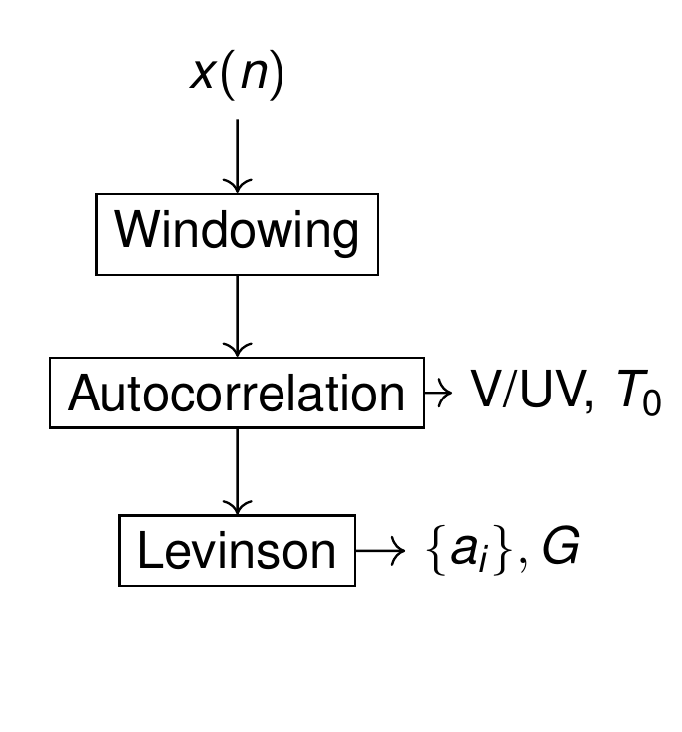
\includegraphics[width=0.75\textwidth]{images/Linear_predictive_coding_-_analysis.png}
\caption{Linear predictive coding - analysis}
\end{figure}\begin{tcolorbox}[colback=white, colframe=gray!50, height=4.5cm, sharp corners]
\end{tcolorbox}

This \textbf{LPC} analysis scheme estimates speech-model parameters frame by frame. Windowing isolates a short quasi-stationary segment, autocorrelation provides statistics plus voiced/unvoiced and \textbf{pitch}-period information, and Levinson-Durbin solves the linear prediction equations to obtain the \textbf{LPC} coefficients $\{a_i\}$ and gain $G$.


\begin{figure}[H]
\centering
\begin{tikzpicture}[
    node distance=1.1cm,
    block/.style={draw, fill=blue!5, text width=7.5cm, align=center, minimum height=0.6cm, rounded corners=3pt, font=\small},
    arrow/.style={thick,->,>=stealth}
]
    \node (a) [block] {Speech Frame ($\sim 20$ ms)};
    \node (b) [block, below=of a] {Windowing};
    \node (c) [block, below=of b] {Autocorrelation};
    \node (d) [block, below=of c] {Levinson-Durbin / Yule-Walker};
    \node (e) [block, below=of d] {LPC Coefficients, Gain, Pitch, Voiced/Unvoiced Decision};

    \draw [arrow] (a) -- (b);
    \draw [arrow] (b) -- (c);
    \draw [arrow] (c) -- (d);
    \draw [arrow] (d) -- (e);
\end{tikzpicture}
\caption{LPC Analysis Block Scheme}
\end{figure}


Prediction model:


$$
\hat{x}(n)=-\sum_{i=1}^{P}a_i x(n-i)
$$


Residual:


$$
y(n)=x(n)-\hat{x}(n)=\sum_{i=0}^{P}a_i x(n-i),\quad a_0=1
$$


Voiced frames use \textbf{pitch}-period excitation; unvoiced frames use noise-like excitation. \textbf{LPC}-10 is low bitrate, but less natural than \textbf{CELP} because its excitation model is too rigid.



\begin{questionbox}{Domanda 45}
(A\&S Comp.) Draw the scheme and describe the operation of the functional blocks of an MP3 encoder.
\end{questionbox}


MP3 is a perceptual audio codec. Its encoder can be summarized as:

\begin{figure}[H]
\centering
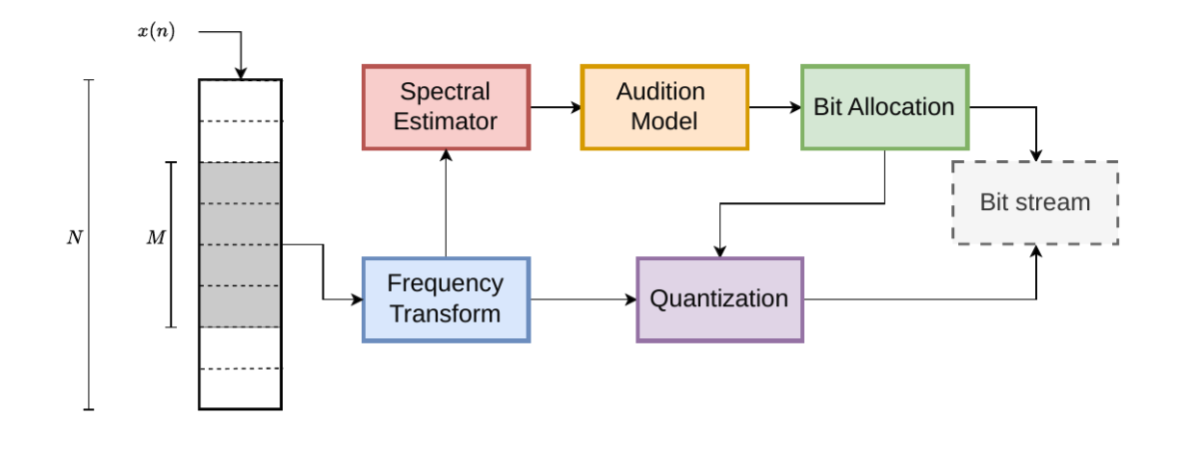
\includegraphics[width=0.75\textwidth]{images/Pasted_image_20260624185047.png}
\caption{Pasted image 20260624185047}
\end{figure}\begin{tcolorbox}[colback=white, colframe=gray!50, height=4.5cm, sharp corners]
\end{tcolorbox}

The \textbf{psychoacoustic model} is encoder-side only. The decoder performs inverse \textbf{quantization} and inverse transform.



\begin{questionbox}{Domanda 46}
(A\&S Comp.) Why are Line Spectrum Frequencies (LSF) preferred over direct \textbf{quantization} of \textbf{LPC} coefficients ($a_i$)?
\end{questionbox}


Direct \textbf{LPC} coefficient \textbf{quantization} can easily create unstable synthesis filters. Line Spectrum Frequencies represent the \textbf{LPC} filter through roots on the unit circle. Stability can be checked and enforced by preserving interlacing/order:


$$
0<\omega_1^{(P)}<\omega_1^{(Q)}<\omega_2^{(P)}<\cdots<\pi
$$


If \textbf{quantization} disturbs the order, the decoder can restore a valid ordering, making stable reconstruction easier.



\begin{questionbox}{Domanda 47}
(A\&S Comp.) Regarding the Opus audio codec, what is the primary technical advantage of its hybrid design?
\end{questionbox}


Opus combines:

\begin{itemize}
  \item \textbf{SILK:} \textbf{LPC}-based, efficient for speech and low bitrates.
  \item \textbf{CELT:} \textbf{MDCT}-based, efficient for music/general audio and low delay.
\end{itemize}

The key advantage is seamless adaptation across speech, music, bitrate and latency constraints, which is useful for WebRTC and real-time communication.



\begin{questionbox}{Domanda 48}
(A\&S Comp.) Which of the following best describes current research trends in the future of multimedia audio coding?
\end{questionbox}


Main trends:

\begin{itemize}
  \item neural speech and audio codecs at very low bitrates,
  \item perceptual and QoE-driven quality metrics,
  \item spatial/immersive audio,
  \item robust real-time coding under latency constraints,
  \item quality assessment for generated or enhanced audio.
\end{itemize}

---


